\section{极限与余极限}

两个重要定义——\trLimit{}与\trColimit——由\trUniversalProperty{}确定。它们把一串熟悉的构造收编为特例。我先给出定义，再向你说明它们为何是你熟悉的东西。例如，分数将是余极限的动机性例子（\cref{ex:rational-union-colimit}(a)），而\trPadicIntegers{}（例~1.3.4）将是极限的动机性例子。

\textbf{1.3.1. 极限。}\quad 若一个\trCategory{}的对象构成一个集合，且其态射也构成一个集合，则称之为\textbf{\trSmallCategory}（small category）。（这是一条技术性条件，本只为行家而设。）设 $\scr{S}$ 是任何小范畴，$\scr{C}$ 是任何范畴。则一个函子 $F\colon\scr{S}\to\scr{C}$（即：对每个元素 $i\in\scr{S}$ 给定一个对象 $\mathrm{A}_i\in\scr{C}$，连同由 $\scr{S}$ 所支配的、恰当交换的诸态射）称为一个以 $\scr{S}$ 为指标的\textbf{\trDiagram}（diagram）。我们称 $\scr{S}$ 为\textbf{\trIndexCategory}（index category）。我们的指标范畴通常将是偏序集（例~1.1.8），其中特别地，任何两个对象之间至多有一个态射。（但别的例子有时也有用。）例如，若 $\square$ 是范畴
\[
\begin{tikzcd}[row sep=1.5em, column sep=2.4em]
\bullet \ar[r] \ar[d] & \bullet \ar[d] \\
\bullet \ar[r] & \bullet
\end{tikzcd}
\]
而 $\scr{A}$ 是一个范畴，则函子 $\square\to\scr{A}$ 恰是 $\scr{A}$ 中一个交换方图的数据。

于是，该\trDiagram{}的\textbf{\trLimit}（limit）是 $\scr{C}$ 的一个对象 $\varprojlim_{\scr{S}}\mathrm{A}_i$（或 $\varprojlim_i\mathrm{A}_i$），连同态射 $\mathrm{f}_j\colon\varprojlim_{\scr{S}}\mathrm{A}_i\to\mathrm{A}_j$（对每个 $j\in\scr{S}$），使得若 $\mathrm{m}\colon j\to k$ 是 $\scr{S}$ 中的态射，则
\begin{equation*}\tag{1.3.1.1}\label{eq:limit-cone-diagram}
\begin{tikzcd}[row sep=2.1em, column sep=3.4em]
 & \varprojlim_{\scr{S}}\mathrm{A}_i \ar[dl,"\mathrm{f}_j"'] \ar[dr,"\mathrm{f}_k"] & \\
\mathrm{A}_j \ar[rr,"F(\mathrm{m})"'] & & \mathrm{A}_k
\end{tikzcd}
\end{equation*}
交换，并且该对象连同到诸 $\mathrm{A}_i$ 的映射关于这条性质是泛的（终的）。更精确地说：给定任何别的对象 $W$ 连同映射 $\mathrm{g}_i\colon W\to\mathrm{A}_i$（与诸 $F(\mathrm{m})$ 交换：若 $\mathrm{m}\colon j\to k$ 是 $\scr{S}$ 中的态射，则 $\mathrm{g}_k=F(\mathrm{m})\circ\mathrm{g}_j$），则存在唯一的映射
\[
\mathrm{g}\colon W\to\varprojlim_{\scr{S}}\mathrm{A}_i
\]
使得 $\mathrm{g}_i=\mathrm{f}_i\circ\mathrm{g}$ 对一切 $i$ 成立。（在某些情形，极限有时称为\trInverseLimit{}（inverse limit）或\trProjectiveLimit{}（projective limit）。我们不用这套语言。）按通常的泛性质论证，极限若存在，便在相差唯一同构的意义下唯一。

\textbf{1.3.2. 例：积。}\quad 例如，若 $\scr{S}$ 是偏序集
\[
\begin{tikzcd}[row sep=2.4em, column sep=3em]
 & & \bullet \ar[d] \\
\bullet \ar[rr] & & \bullet
\end{tikzcd}
\]
我们便得到\trFiberProduct。若 $\scr{S}$ 是
\[
\begin{tikzcd}
\bullet & \bullet
\end{tikzcd}
\]
我们便得到\trProduct。

若 $\scr{S}$ 是一个集合（即其态射仅有恒等映射），则该极限称为诸 $\mathrm{A}_i$ 的\trProduct，记作 $\prod_i\mathrm{A}_i$。$\scr{S}$ 有两个元素的特殊情形，正是上一段的例子。

\begin{exercise}[现实检验]\label{ex:initial-object-limit}
假设偏序集 $\scr{S}$ 有一个\trInitialObject{} $e$。证明：任何以 $\scr{S}$ 为指标的\trDiagram{}之极限都存在。
\end{exercise}

\begin{exercise}[再论对角—基变换图]\label{ex:basechange-diagonal-limit}
把 $X_1\times_Y X_2$ 与 $Y\times_{(Y\times_Z Y)}(X_1\times_Z X_2)$ 都认同为下图
\[
\begin{tikzcd}[row sep=1.8em, column sep=2.6em]
\mathrm{X}_1 \ar[dr] & & \\
 & \mathrm{Y} \ar[r] & \mathrm{Z} \\
\mathrm{X}_2 \ar[ur] & &
\end{tikzcd}
\]
的极限，从而把\cref{ex:diagonal-base-change-square}再做一遍。
\end{exercise}

\textbf{1.3.3. 例：\trFormalPowerSeries。}\quad 对环 $\Lambda$，\textbf{\trFormalPowerSeries}（(formal) power series）$\Lambda[[x]]$ 常被非正式地（而且有点不自然地）描述为环
\[
\Lambda[[x]]=\{a_0+a_1x+a_2x^2+\cdots\}
\]
（其中 $a_i\in\Lambda$，环运算取「显然」的那些）。它是环的范畴中极限的一个例子：
\[
\begin{tikzcd}[row sep=1.9em, column sep=2.1em]
\Lambda[[x]] \ar[dr] \ar[drr] \ar[drrr] & & & & \\
 & \cdots \ar[r] & \Lambda[x]/(x^3) \ar[r] & \Lambda[x]/(x^2) \ar[r] & \Lambda[x]/(x)
\end{tikzcd}
\]
极限的\trUniversalProperty{}给出一个自然的环映射 $\Lambda[x]\to\Lambda[[x]]$。若 $\Lambda=\mathbb{R}$ 或 $\mathbb{C}$，此映射穿过由\trConvergentPowerSeries{}组成的环。

\textbf{1.3.4. 例：\trPadicIntegers。}\quad 对素数 $p$，\textbf{\trPadicIntegers}（$p$-adic integers；更非正式的说法是 \trPadics）$\mathbb{Z}_p$ 常被非正式地（而且有点不自然地）描述为形如
\[
a_0+a_1p+a_2p^2+\cdots
\]
的东西（其中 $0\le a_i<p$）。它们是环的范畴中极限的一个例子：
\[
\begin{tikzcd}[row sep=1.9em, column sep=2.1em]
\mathbb{Z}_p \ar[dr] \ar[drr] \ar[drrr] & & & & \\
 & \cdots \ar[r] & \mathbb{Z}/(p^3) \ar[r] & \mathbb{Z}/(p^2) \ar[r] & \mathbb{Z}/(p)
\end{tikzcd}
\]
（警示：$\mathbb{Z}_p$ 有时用来指模 $p$ 的整数，但为免混淆，这种场合最好用 $\mathbb{Z}/(p)$ 或 $\mathbb{Z}/p\mathbb{Z}$。更糟的是：按 \S1.2.3，$\mathbb{Z}_p$ 又表示分母为 $p$ 的幂的那些有理数。但愿 $\mathbb{Z}_p$ 的含义在语境中总是清楚的。）

例 1.3.3 与例 1.3.4 的相似绝非巧合。形式幂级数与 $p$~进整数都是\textbf{\trCompletion}（completion）的例子——那是第 28 章的主题。

极限并不对任何\trIndexCategory{} $\scr{S}$ 都存在。不过，若你的范畴中的对象可以解释成带附加结构的集合，且任意\trProduct{}都存在（并尊重这种「集合式」的结构），你往往就能轻松验证极限存在。

\begin{exercise}[重要练习]\label{ex:elementwise-limit-description}
证明：在范畴 $\catSets$ 中，
\[
\left\{(\mathrm{a}_i)_{i\in\scr{S}}\in\prod_i\mathrm{A}_i:\ F(\mathrm{m})(\mathrm{a}_j)=\mathrm{a}_k\ \text{对一切}\ \mathrm{m}\in\Mor_{\scr{S}}(j,k)\subset\Mor(\scr{S})\right\},
\]
连同到每个 $\mathrm{A}_i$ 的显然投射映射，就是极限 $\varprojlim_{\scr{S}}\mathrm{A}_i$。

这在 $\Lambda$-模范畴 $\catMod{\Lambda}$（特别是 $\catVec_k$ 与 $\catAb$）中显然同样成立，在 $\catRings$ 中亦然。由此观点看，$2+3p+2p^2+\cdots\in\mathbb{Z}_p$ 可以理解为序列 $(2,\,2+3p,\,2+3p+2p^2,\dots)$。
\end{exercise}

\textbf{1.3.5. 余极限。}\quad 对我们更直接有用的，将是极限（或\trInverseLimit）观念的对偶（箭头反转的版本）。只要把\eqref{eq:limit-cone-diagram}中的箭头 $\mathrm{f}_i$ 翻转，便得到\textbf{\trColimit}（colimit）的观念，记作 $\colim_{\to\scr{S}}\mathrm{A}_i$（或 $\lim\nolimits_{\to\scr{S}}\mathrm{A}_i$）。（相应的图请你自行画出。）同样，它若存在，便在相差唯一同构的意义下唯一。（在某些情形，余极限有时称为\trDirectLimit{}（direct limit）、\trInductiveLimit{}（inductive limit）或\trInjectiveLimit{}（injective limit）。我们不用这套语言。我更愿意借核／余核、积／余积的类比来使用极限／余极限。这不只是类比：核与积可以解释为极限，余核与余积亦然。而且我记得：核是「映过去」的，余核是「被映过来」的——这提醒我：极限映到以 $\scr{S}$ 为指标的那个大交换图中的所有对象，而余极限则有来自图中所有对象的映射。）

\textbf{1.3.6. 笑话。}\quad \trComathematician{}是一种把余定理变成 ffee 的装置。%
\footnote{译注：原文戏言：数学家（mathematician）把咖啡（coffee）变成定理（theorems）；对偶地，「\trComathematician」（comathematician）把「余定理」（cotheorems）变成 ffee——coffee 去掉前缀 co- 便是 ffee。}

尽管只是把箭头翻了过来，余极限的表现却与极限颇为不同。

\textbf{1.3.7. 例。}\quad 分母为 $5$ 的幂的有理数组成的阿贝尔群 $5^{-\infty}\mathbb{Z}$ 是一个余极限 $\colim_{i\in\mathbb{Z}_+}5^{-i}\mathbb{Z}$。更精确地说，$5^{-\infty}\mathbb{Z}$ 是图
\[
\mathbb{Z}\longrightarrow 5^{-1}\mathbb{Z}\longrightarrow 5^{-2}\mathbb{Z}\longrightarrow\cdots
\]
在阿贝尔群范畴中的余极限。

在\trIndexSet{} $\scr{S}$ 上取的余极限称为\textbf{\trCoproduct}（coproduct），记作 $\coprod_i\mathrm{A}_i$，它是积的对偶（箭头反转）观念。

\begin{exercise}\label{ex:rational-union-colimit}
\begin{enumerate}[label=(\alph*)]
\item 解释命题「$\mathbb{Q}=\colim\frac{1}{n}\mathbb{Z}$」。
\item 把给定集合的若干子集之并解释为一个余极限。（对偶地，交可以解释为极限。）此处所论范畴的对象是该给定集合的诸子集。
\end{enumerate}
\end{exercise}

余极限并不总存在，但有两类有用的大类例子，在其中存在。

\textbf{1.3.8. 定义。}\quad 非空偏序集 $(S,\ge)$ 称为\textbf{\trFiltered{}的}（filtered），或称\textbf{\trFiltered{}集}（filtered set），若对每个 $x,y\in S$，存在 $z$ 使 $x\ge z$ 且 $y\ge z$。更一般地（见图~1.1），非空范畴 $\scr{S}$ 称为\trFiltered{}的，若：（i）对每个 $x,y\in\scr{S}$，存在 $z\in\scr{S}$ 及箭头 $x\to z$ 与 $y\to z$；且（ii）对每两个箭头 $u\colon x\to y$ 与 $v\colon x\to y$，存在箭头 $w\colon y\to z$ 使 $w\circ u=w\circ v$。（别的术语也常见，如「\trDirected{}偏序集」与「\trFiltered{}指标范畴」，分别对应这两种情形。）

\begin{figure}[htbp]
  \centering
  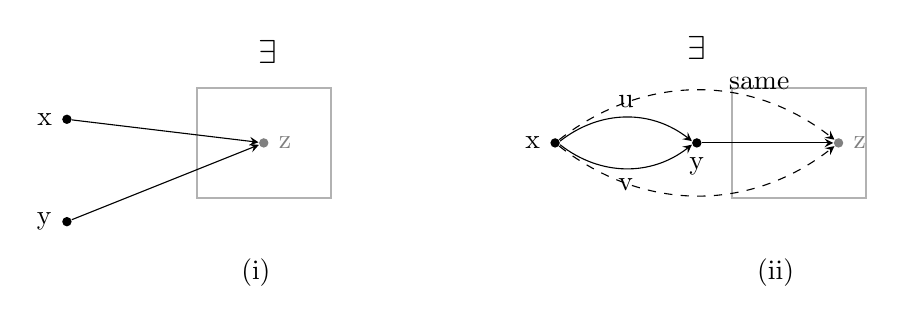
\begin{tikzpicture}[>=stealth,
    dot/.style={circle,fill,inner sep=1.2pt},
    gdot/.style={circle,fill=gray,inner sep=1.2pt}]
    \begin{scope}
      \node at (1.05,1.9) {\large $\exists$};
      \draw[gray!60,semithick] (0.15,0.05) rectangle (1.85,1.45);
      \node[gdot,label={[gray]0:$\mathrm{z}$}] (z) at (1.0,0.75) {};
      \node[dot,label={180:$\mathrm{x}$}] (x) at (-1.5,1.05) {};
      \node[dot,label={180:$\mathrm{y}$}] (y) at (-1.5,-0.25) {};
      \draw[->] (x) -- (z);
      \draw[->] (y) -- (z);
      \node at (0.9,-0.9) {(i)};
    \end{scope}
    \begin{scope}[xshift=6.4cm]
      \node at (0.1,1.95) {\large $\exists$};
      \draw[gray!60,semithick] (0.55,0.05) rectangle (2.25,1.45);
      \node[gdot,label={[gray]0:$\mathrm{z}$}] (z) at (1.9,0.75) {};
      \node[dot,label={180:$\mathrm{x}$}] (x) at (-1.7,0.75) {};
      \node[dot,label={-90:$\mathrm{y}$}] (y) at (0.1,0.75) {};
      \draw[->] (x.20) to[bend left=38] node[above]{$\mathrm{u}$} (y.160);
      \draw[->] (x.-20) to[bend right=38] node[below]{$\mathrm{v}$} (y.200);
      \draw[->] (y) -- (z);
      \draw[->,dashed] (x) to[bend left=38] node[above,pos=0.72]{\text{same}} (z);
      \draw[->,dashed] (x) to[bend right=38] (z);
      \node at (1.1,-0.9) {(ii)};
    \end{scope}
  \end{tikzpicture}
  \caption{\trFiltered{}范畴（图画式定义）。}
\end{figure}

\begin{exercise}\label{ex:filtered-colimit-formula}
设 $\scr{S}$ 是\trFiltered{}的。（我们几乎只用 $\scr{S}$ 为\trFiltered{}集的情形。）回忆 $\coprod$ 表示集合的\trDisjointUnion。证明：$\catSets$ 中任何以 $\scr{S}$ 为指标的\trDiagram，连同到它的显然映射，有如下余极限：
\[
\Bigl\{(\mathrm{a}_i,i)\in\coprod_{i\in\scr{S}}\mathrm{A}_i\Bigr\}\Bigg/
\Bigl(\begin{array}{l}
(\mathrm{a}_i,i)\sim(\mathrm{a}_j,j)\ \text{当且仅当图中存在 }\mathrm{f}\colon\mathrm{A}_i\to\mathrm{A}_k\text{ 与 }\mathrm{g}\colon\mathrm{A}_j\to\mathrm{A}_k\\[2pt]
\text{使得在 }\mathrm{A}_k\text{ 中 }\mathrm{f}(\mathrm{a}_i)=\mathrm{g}(\mathrm{a}_j)
\end{array}\Bigr)
\]
（你会看到，「滤过」假设正是为了保证 $\sim$ 是\trEquivalenceRelation。）
\end{exercise}

例如在例 1.3.7 中，余极限的每个元素都是「楼上」某个东西里的元素，只是你无法预先说出它是哪个东西里的元素。例如，$17/125$ 是 $5^{-3}\mathbb{Z}$（或 $5^{-4}\mathbb{Z}$，或更靠后的）中的元素，但不是 $5^{-2}\mathbb{Z}$ 中的元素。

这个想法适用于对象可以解释成带附加结构的集合的许多范畴（如阿贝尔群、$\Lambda$-模、群等）。例如，$\Lambda$-模范畴 $\catMod{\Lambda}$ 中的余极限 $\colim M_i$ 可以如下描述。$\colim M_i$ 的底集合按\cref{ex:filtered-colimit-formula}定义。要把元素 $\mathrm{m}_i\in M_i$ 与 $\mathrm{m}_j\in M_j$ 相加，选取 $\ell\in\scr{S}$ 及箭头 $u\colon i\to\ell$ 与 $v\colon j\to\ell$，然后把 $\mathrm{m}_i$ 与 $\mathrm{m}_j$ 之和定义为 $F(u)(\mathrm{m}_i)+F(v)(\mathrm{m}_j)\in M_\ell$。元素 $\mathrm{m}_i\in M_i$ 为 $0$，当且仅当存在某支箭头 $u\colon i\to k$ 使 $F(u)(\mathrm{m}_i)=0$，也就是说，当且仅当它在「图的更靠后处」变成 $0$。最后，用 $\Lambda$ 的元素作乘法按显然的方式定义。

\begin{exercise}\label{ex:module-colimit-verification}
验证上面描述的 $\Lambda$-模确实是余极限。（务必验证加法是\trWellDefined{}的，即它不依赖于代表元 $\mathrm{m}_i$ 与 $\mathrm{m}_j$ 的选取、$\ell$ 的选取，以及箭头 $u$ 与 $v$ 的选取。同样务必验证数乘是\trWellDefined{}的。）
\end{exercise}

\begin{exercise}[有用练习：局部化作为余极限]\label{ex:localization-as-colimit}
把\cref{ex:rational-union-colimit}(a)推广，把\trIntegralDomain{}的局部化解释为\trFiltered{}集上的余极限：设 $S$ 是 $\Lambda$ 的\trMultiplicativeSubset，并解释 $S^{-1}\Lambda=\colim\frac{1}{s}\Lambda$，其中余极限在 $s\in S$ 上取，且在 $\Lambda$-模范畴中取。（旁注：若 $\Lambda$ 不是\trIntegralDomain，你能否使这套做法的某个版本奏效，例如 $S^{-1}\Lambda=\colim\Lambda_s$？这将在 $\Lambda$-\trAlgebra{}的范畴中奏效。）
\end{exercise}

若你有别的办法「连接图中不同对象里的元素」，上述构造有一个不要滤过条件的变体。例如：

\begin{exercise}[练习：无滤过条件的 $\Lambda$-模余极限]\label{ex:unfiltered-module-colimit}
设有以 $\scr{S}$ 为指标的 $\Lambda$-模\trDiagram{} $F\colon\scr{S}\to\catMod{\Lambda}$，记 $M_i:=F(i)$。证明：余极限是 $\bigoplus_{i\in\scr{S}}M_i$ 模去关系 $\mathrm{m}_i-F(n)(\mathrm{m}_i)$（对 $\scr{S}$ 中每个 $n\colon i\to j$，即图中每支箭头）。（说得稍精确些：「模去」意指「对由其生成的\trSubmodule{}取\trQuotient」。）
\end{exercise}

\textbf{1.3.9. 小结。}\quad 非正式地，把下面这件事放在心里是有用的。在对象是「集合式的」范畴中，极限的一个元素可以想成图中每个对象的一族彼此「相容」的元素（\cref{ex:elementwise-limit-description}）；而余极限的一个元素则可视为图中单个对象里的一个元素（「即它有一个代表元恰好是」这样的元素）（\cref{ex:filtered-colimit-formula}）。极限与余极限的定义虽只差箭头反转，这些解释却大异其趣。

\textbf{1.3.10. 小注记。}\quad 事实上，对所有合理的（「小」）指标范畴，集合范畴中的余极限都存在（例如见 [E, Thm.~A6.1]），但这与我们无关。

\textbf{1.3.11. 笑话。}\quad 读一篇范畴论论文的人，怎么称呼？答案：\trCoauthor{}（coauthor）%
\footnote{译注：原文玩「co-」前缀梗：只读不写的人被戏称为 coauthor（共同作者）；仿余极限（colimit）、余核（cokernel）的「余」字，戏译作「余作者」。}。

